\chapter{Problem Statement}
\label{chap:problem_statement}

\section{Context}
\label{sec:context}

\section{Work Environment}
\label{sec:work_environment}

This project was done within the framework of the Master 2 Computer Science program at the 
\textbf{Laboratoire de Mathématiques Informatique et Applications (LAMIA)} of the \textbf{Université des Antilles}.
The following tools and technologies were used to develop the algorithms and document the project:

\begin{itemize}
	\item \textbf{Python}: a programming language widely used in scientific computing, data analysis, and machine learning.
	\item \textbf{GitHub}: a version control platform for managing the source code.
	\item \textbf{Jupyter Notebook}: an interactive environment for writing and executing Python code, ideal for data analysis and 
	visualization.
	\item \textbf{sklearn}: a Python library for machine learning that provides various algorithms and tools for data preprocessing, 
	model selection, and evaluation.
	\item \LaTeX : a typesetting system used for writing technical and scientific documents.
	\item A personal computer running Windows 11 with a \textbf{Ryzen 7 6800H} processor and \textbf{32 GB} of RAM.
\end{itemize}

\section{Objectives}
\label{sec:objectives}

\chapter{Genomic data}
\label{chap:genomic_data}


\section{The FASTA format}
\label{sec:fasta_format}

\section{From a genome to an image}
\label{sec:genome_to_image}

\chapter{Clustering genomic data}
\label{chap:clustering_genomic_data}

\section{Introduction to K-means}
\label{sec:intro_kmeans}

K-means clustering is a widely used unsupervised learning algorithm for partitioning a dataset into $k$ distinct clusters.
It works by iinitializing $k$ cluster centers, then iteratively assigning data points to the nearest cluster center and 
updating the centers based on the distances to the assigned points (usually using Euclidean distance). The algorithm 
continues until the cluster centers stabilize or a maximum number of iterations is reached.

Results can vary based on the initial choice of cluster centers, which can lead to different clustering outcomes. 
The quality of clusters is typically evaluated using at least two criteria:

\begin{itemize}
	\item \textbf{Intra-cluster variance} : the average distance between points within the same cluster.
	\item \textbf{Inter-cluster variance} : the average distance between centers of different clusters.
\end{itemize}

\subsection{K-means Algorithm}
\label{subsec:kmeans_algorithm}

The K-means algorithm consists of the following steps:
\begin{enumerate}
	\item Initialize $k$ cluster centers randomly.
	\item Assign each data point to the nearest cluster center.
	\item Update the cluster centers by calculating the mean of the points assigned to each cluster.
	\item Repeat steps 2 and 3 until convergence (i.e., when cluster centers do not change significantly).
	\item Optionally, evaluate the clustering quality using metrics like inertia or silhouette score.
\end{enumerate}

\section{Silhouette Score}
\label{subsec:silhouette_score}

The silhouette score is a metric used to evaluate the quality of clustering. It measures how similar an object 
is to its own cluster compared to other clusters. The silhouette score is calculated for each data point and
ranges from -1 to 1. The formula for the silhouette score of a point $i$ is:

\begin{equation}
	s(i) = \frac{b(i) - a(i)}{\max(a(i), b(i))}
\end{equation}

Where $a(i)$ is the average distance from point $i$ to all other points in the same cluster, and $b(i)$ is the
average distance from point $i$ to all points in the nearest cluster. A higher silhouette score indicates better 
clustering quality.

\section{Principal Component Analysis (PCA)}
\label{subsec:pca}



\section{Preprocessing Genomic Data}
\label{sec:preprocessing_genomic_data}

Our data is a collection of Tuberculosis (TB) genomes, where each file contains the proteins and their respective
nucleotide sequences in FASTA format, for a total of 7057 files.
TODO: parler de l'institut Pasteur?
The goal is to cluster these genomes based on their protein sequences and find ways to distinguish between different
TB strains.

We started by creating a dataset containing the number of times each protein appears in each genome. This was done by 
parsing the FASTA files and counting the occurrences of each protein sequence, we then removed the outliers, namely
"hypothetical proteins" and "putative proteins", which are not well characterized and do not provide useful information
for clustering. The resulting dataset is a CSV of 7057 columns plus 1 column for the protein names and 2732 rows plus 1
row for header.

Considering the size of the dataset, we used Principal Component Analysis (PCA) set to 95\% variance to reduce the dimensionality
of the data while preserving as much variance as possible. PCA is a technique that transforms the data into a new coordinate 
system, where the first principal component captures the maximum variance, the second captures the second maximum variance, 
and so on.

We then calculated the silhouette score for different values of $k$, ranging from 2 to 10, to determine the optimal number 
of clusters. The silhouette score was calculated using the `silhouette_score` function from the `sklearn.metrics` module, 
which takes the data and the cluster labels as input. The optimal number of clusters is the one that maximizes the silhouette
score. 

\subsection{First Results}
\label{subsec:first_results}

The initial results showed that the silhouette score was highest for $k=9$, indicating that this was the optimal number of clusters.
However, the clusters were not well separated or some points are alone in their cluster, as seen in Figure {TODO:figure:clusters_k9}.
Which suggests that the data may not be well suited for clustering with K-means, or that the features used for clustering are not 
informative enough. We also tried without PCA but achieved similar results, we also observed a fewer points than expected as seen in
Figure {TODO:figure:clusters_k9_no_pca}, after reviewing the data, we found that there is significant overlap between the points.

TODO: figure clusters_k9

TODO: figure clusters_k9_no_pca

\section{New Approach using DBSCAN and HDBSCAN}
\label{subsec:new_approach_dbscan_hdbscan}

To address the limitations of K-means clustering, we explored alternative clustering algorithms, specifically 
\textbf{DBSCAN} and \textbf{HDBSCAN}.

DBSCAN (Density-Based Spatial Clustering of Applications with Noise) is a density-based clustering algorithm that
groups points that are close together based on a distance measurement and a minimum number of points. It is particularly 
effective for datasets with varying densities and can identify noise points that do not belong to any cluster.

HDBSCAN (Hierarchical Density-Based 
Spatial Clustering of Applications with Noise) is an extension of DBSCAN that builds a hierarchy of clusters and allows for
more flexible clustering by varying the density threshold. It can also handle varying cluster shapes and sizes.

TODO

\subsection{Principle}
\label{subsec:principle_dbscan_hdbscan}

\subsection{Results}
\label{subsec:results_dbscan_hdbscan}

\section{Trying an autoencoder}
\label{sec:autoencoder}

\chapter{Using CNNs to identify TB Strains}
\label{chap:cnn_tb_strains}

\section{Introduction to CNNs}
\label{sec:intro_cnn}

The fondamental idea behind \textbf{Convolutional Neural Networks (CNNs)} was introduced by Kunihiko Fukushima~\cite{Fukushima-1987}
in 1980 and later popularized by Yann LeCun in the 1990s with the LeNet architecture. CNNs are a class of deep learning 
models specifically designed for processing structured grid data, such as images.  They are particularly effective for tasks 
like image classification, object detection, and segmentation.

CNNs work by applying convolutional filters to the input data, which allows them to learn spatial hierarchies of features.
It shares some similarities with the more conventional neural networks, but there is at least two different types
of layers that are specific to CNNs:

\begin{itemize}
	\item \textbf{Convolutional layers}: These layers apply convolutional filters to the input data, extracting local features 
	that are invariant to translation. The filters slide over the input data, computing dot products and producing feature maps.
	\item \textbf{Pooling layers}: These layers downsample the feature maps, reducing their spatial dimensions while retaining important 
	information. Common pooling operations include max pooling and average pooling.
\end{itemize}

The architecture of a CNN typically consists of multiple convolutional and pooling layers followed by fully connected layers.
The convolutional layers learn to extract features from the input data, while the fully connected layers perform the final classification
or regression task. The training process involves optimizing the weights of the filters and fully connected layers using backpropagation
and a loss function, such as cross-entropy for classification tasks.

\section{Building the dataset}
\label{sec:building_dataset}

For this experiment, each genome was converted into an image where each pixel is determined by a combination of three metrics of following
metrics:

\begin{itemize}
	\item \textbf{Chargaff}
	\item \textbf{Composition}
	\item \textbf{Diversity}
	\item \textbf{Skew}
	\item \textbf{Nuclescore}
\end{itemize}

We get ten combinations of these metrics, each represented by a different color channel in the image. We applied this conversion at different 
resolutions, from 4px (2x2) to 100px (10x10), the resulting images put into their corresponding class based on the strain they belong to. We 
have the following classes:

\begin{itemize}
	\item \textbf{M} with 185 samples.
	\item \textbf{East Asian} with 1651 samples.
	\item \textbf{East-African Indian} with 267 samples.
	\item \textbf{Euro-American} with 4409 samples.
	\item \textbf{Indo-Oceanic} with 259 samples.
\end{itemize}


\subsection{Initial testing}
\label{subsec:initial_testing}

The resulting dataset is highly imbalanced, with some classes having significantly more samples than others. This can lead to biased models 
that perform poorly on minority classes. We decided to train our CNN on the dataset as-is, without any preprocessing or balancing techniques,
to see how it performs on the imbalanced dataset. 

\section{Mitigating class imbalance}
\label{sec:mitigating_class_imbalance}

We have multiple ways of addressing the class imbalance issue in our dataset, including:
\begin{itemize}
	\item Cross validation
	\item Under-sampling
	\item Data augmentation
	\item Combining under-sampling and data augmentation
\end{itemize}

We will explore each of these techniques in the following sections and compare the results to see which one yields the best performance.

\subsection{Cross validation}
\label{subsec:cross_validation}

Cross validation is a technique used to evaluate the performance of a model by splitting the dataset into multiple subsets, or folds.
The model is trained on a subset of the data and tested on the remaining data, and this process is repeated for each fold. 
This allows for a more robust evaluation of the model's performance, as it reduces the risk of overfitting to a specific subset of the data.
\subsubsubsection{K-fold cross validation}
\label{subsubsec:k_fold_cross_validation}

K-fold cross validation is a specific type of cross validation where the dataset is divided into $k$ equally sized folds. The model is trained 
on $k-1$ folds and tested on the remaining fold, and this process is repeated for each fold. The final performance is averaged over all folds 
to obtain a more reliable estimate of the model's performance. The graphical representation of K-fold cross validation is shown in Figure~\ref{fig:k_fold}.

\begin{figure}[htbp]
	\centering
	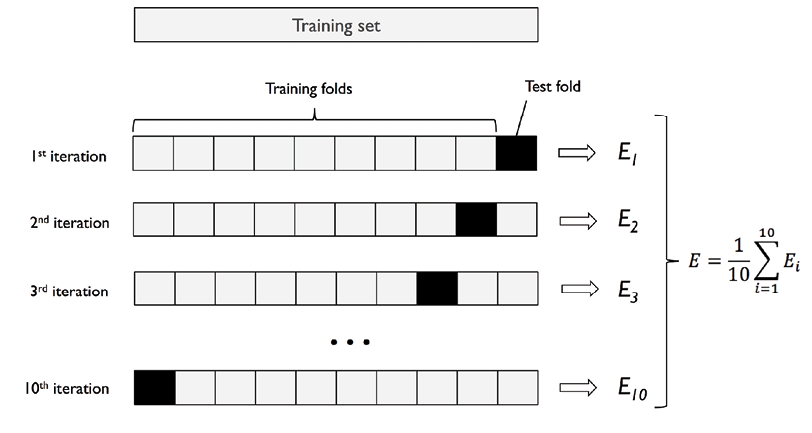
\includegraphics[width=0.8\textwidth]{../imgs/kfold.png}
	\caption{How K-fold cross validation works.\cite{Raschka-Mirjalili-2017}}
	\label{fig:k_fold}
\end{figure}


\subsubsubsection{Stratified K-fold cross validation}
\label{subsubsec:stratified_k_fold_cross_validation}

Stratified K-fold cross validation is a variation of K-fold cross validation that ensures that each fold has the same proportion of samples 
from each class. This is particularly useful for imbalanced datasets, as it ensures that each fold has a representative sample of each class.
Even if this method is recommended for imbalanced datasets, we did not have enough time to implement it, so we used the standard K-fold cross validation.

\subsubsubsection{Remaking the dataset}
\label{subsubsec:remaking_dataset}

\subsection{Under-sampling}
\label{subsec:under_sampling}

\subsection{Data augmentation}
\label{subsec:data_augmentation}

\subsubsubsection{SMOTE}
\label{subsubsec:smote}

Synthetic Minority Over-sampling Technique (SMOTE) is a popular technique for generating synthetic samples in imbalanced datasets.

\subsection{Combining techniques}
\label{subsec:combining_techniques}